\section{Results}
\label{sec:results}

In this section, I apply DEQNs to specific variations of ACE, namely with the DICE 2016 and 2023 production function as well as using the typical DICE carbon cycles. Because of the project's scope, I want to note that the results in this section are preliminary and that there has not been a focus on calibrating the model, only solving a model with a given set of parameters. The parameters used for the simulations can be found in the appendix (\ref{apdx:simulation-initializations}), and supplementary figures are presented in the appendix (\ref{appendix:supplementary_figures}). First, the section covers the architecture of the policy network used for approximating the equilibrium conditions, the training scheme used to train it, and error statistics in the equilibrium conditions. Then, I will go on to compare the estimates of the consumption rates and abatement rates with the analytical solutions.


\subsection{Network Architecture and Hyperparameters}

\subsubsection{Network}
As outlined in section (\ref{subsec:model_based_optimal_control}), the policy network used by DEQNs is a Multilayer Perceptron (MLP), consisting solely of densely connected layers. The specific architecture employed in this thesis follows those of the works by \textcite{Azinovic2022DEQN, friedl2023_deepUQ, Folini2024ClimateInCE}\footnote{\textcite{Folini2024ClimateInCE} does not cover the specific architecture for their policy network in the paper. However, they have a GitHub repository accompanying the paper.}. Table (\ref{table:Network_Architecture}) lists each layer with the respective characteristics, and figure (\ref{fig:pol-net-architecture}) is an illustration of the architecture. 

\begin{table}[ht]
\centering
\begin{tabular}{llll}
    \toprule
    Layer Number & Layer Type & Nodes & Activation Function \\
    \midrule
    1 & Input Layer & \(|\mathcal{S}|=7\) & None \\
    2 & Dense & 1024 & ReLu \\
    3 & Dense & 1024 & ReLu \\
    4 & Output Layer & \(|\mathcal{A}|=11\) & Action Specific \\
    \bottomrule
\end{tabular}
\caption{Network Architecture}
\label{table:Network_Architecture}
\end{table}

The input layer takes the state vector, which in the case of the DICE variations of ACE has a state space that is given by \(\bm{s}_t \in \mathbb{R}^7\). Therefore, the size of the input layer is 7. This is followed by two hidden layers, each comprising 1024 neurons. These layers utilize the ReLU (Rectified Linear Unit) activation function. The output layer gives the action vector, which in the case of the DICE variations of ACE is \(\bm{a}_t \in \mathbb{R}^{11}\), meaning that it has 11 units. These outputs are then fed to specific activation functions that map the raw output of the MLP to the appropriate ranges.

\textcite{friedl2023_deepUQ} distinguishes itself from the other papers by using the self-normalizing Scaled Exponential Linear Unit (selu) activation function \parencite{klambauer2017selfnormalizing} in the hidden layers. However, in the interest of simplicity and computational efficiency, I followed the approach of the other two papers and used the relu activation function. The relu function has performed well in previous studies and is easier to compute.

\begin{figure}[ht]
    \centering
    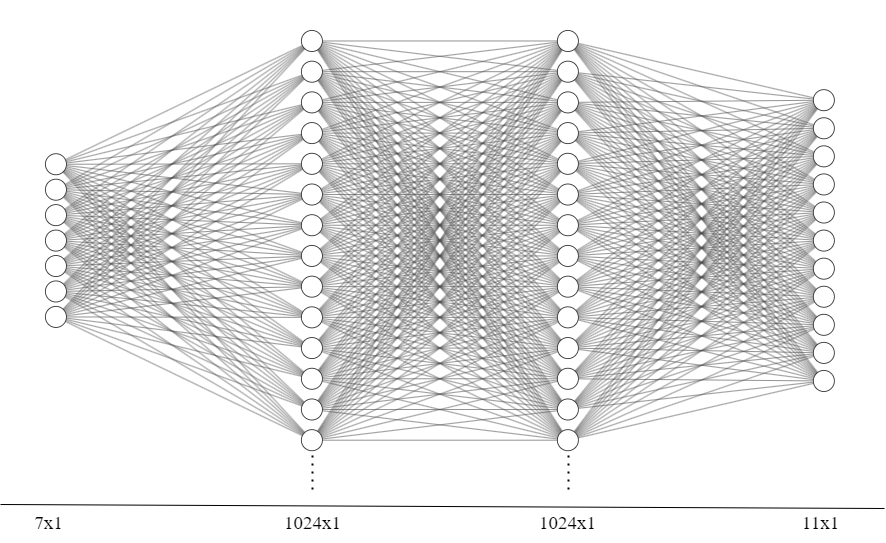
\includegraphics[width=0.9\textwidth]{images/ch6/pol-net-architecture.png}
    \caption{Illustration of policy network architecture}
    \label{fig:pol-net-architecture}
\end{figure}

The output layer has specific activation functions tailored to each action variable. The same custom activation functions were utilized in the output layer in both model runs, as detailed in Table (\ref{table:Custom_Activation_Functions}). The activation functions applied to the costate variables largely mirror those found in \textcite{Folini2024ClimateInCE}, where a linear activation function is applied to each respective costate variable. Each linear output is multiplied by a fixed scale \(c\) that matches the order of magnitude of the variable, so that the network itself only has to produce numbers of order one.

\begin{table}[ht]
\centering
\begin{tabular}{lll}
    \toprule
    Action Variable & Activation Function & Function Mappings \\
    \midrule
    \(x_t\) & Custom Sigmoid & \(f: \mathbb{R} \to (\alpha, 1-\alpha)\), \(\alpha\) small \\
    \(E_t\) & Custom Sigmoid & \(f: \mathbb{R} \to (\alpha, E_t^\text{BAU}(1-\alpha))\), \(\alpha\) small \\ 
    \(V_t\) & Scaled linear, \(c_V = 30\) & \(f: \mathbb{R} \to (-\infty, \infty)\) \\ 
    \(\lambda_{k,t}\) & Linear, \(c_k = 1\) & \(f: \mathbb{R} \to (-\infty, \infty)\) \\
    \(\bm{\lambda}_{M,t}\) & Scaled linear, \(c_M = 10^{-4}\) & \(f: \mathbb{R} \to (-\infty, \infty)\) \\
    \(\bm{\lambda}_{\tau,t}\) & Scaled linear, \(c_\tau = 10^{-1}\) & \(f: \mathbb{R} \to (-\infty, \infty)\) \\
    \(\lambda_{E,t}, \lambda_t^{\text{BAU}}\) & Scaled linear, \(c_{\text{KKT}} = 10^{-4}\) & \(f: \mathbb{R} \to (-\infty, \infty)\) \\
    \bottomrule
\end{tabular}
\caption{Custom Functions}
\label{table:Custom_Activation_Functions}
\end{table}

To prevent potential issues such as taking the logarithm of zero or dividing by zero, modifications were necessary for the activation functions of the control variables \(x_t\) and \(E_t\)\footnote{Refer to appendix (\ref{appendix:deqn_model_specific_mapping}) for the specific functional forms of the two model versions of ACE.}. The custom sigmoid functions scale inputs between a minimal constant \(\alpha\) and an adjusted upper limit \(b\), as depicted in the following equation:

\begin{equation}
    f(x) = b \left( \alpha + (1-2\alpha)\text{sigmoid}(x) \right)
\end{equation}

The custom sigmoid function on \(x_t\) uses \(b=1\) and the custom sigmoid function on \(E_t\) uses \(b=E_t^\text{BAU}\) in both versions, while land-use emissions \(E_t^\text{land}\) enter the carbon cycle exogenously. The bounded emissions are computed once from the raw network output, and the same value is used in the equations of motion and in every objective function.

\subsubsection{Scaling of the Objective Functions}
\label{subsubsec:objective_scaling}

The costate variables differ by several orders of magnitude. At the analytical solution, \(\lambda_{k} \approx 0.35\), while \(\lambda_{M_1} \approx -10^{-4}\). The residuals of the conditions involving the carbon costates are correspondingly small, so in an unweighted sum of squares the carbon conditions \(\ell_1\) and the emissions condition \(\ell_4\) would barely affect the policy objective, and the network could leave the SCC almost undetermined. I therefore divide each residual by the scale of the costate it pins down: \(\ell_1\) and \(\ell_4\) by \(c_M\), and \(\ell_2\) by \(c_\tau\). The Fischer-Burmeister functions are evaluated on the scale-free pairs \((\lambda_{E,t}/c_{\text{KKT}},\, E_t/E_t^\text{BAU})\) and \((\lambda^\text{BAU}_t/c_{\text{KKT}},\, 1 - E_t/E_t^\text{BAU})\). Dividing a residual by a positive constant changes neither its root nor the solution of the system, only how strongly each condition is weighted in the policy objective (eq. \ref{eq:total_objective_function}).


\subsubsection{Training Scheme}

\textcite{friedl2023_deepUQ} implemented a training scheme characterized by a gradual increase in episode length as the policy network stabilized in learning. It started with an episode length of 4 and increased in powers of two, where they, in the final step, went to 300 steps. Furthermore, they used a learning rate of 1e-5 throughout the whole training process. Minibatches were adjusted from 64 to 128 as the network became more stable.

In contrast, the publication by \textcite{Folini2024ClimateInCE} does not provide explicit details on their training methods. However, analysis of their code indicates a similar learning rate of 1e-5, complemented by gradient clipping at a maximum value of 1.0—a technique not mentioned in \textcite{friedl2023_deepUQ}. Their approach also involves increasing episode lengths but not starting as low as in the former study, with lengths set at 50, 100, and 500 steps. Additionally, the initial training cycles consist of 1,000 iterations, escalating to a final cycle of 10,000 iterations.

\begin{table}[ht]
\centering
\begin{adjustbox}{width=\textwidth,center}
{
\begin{tabular}{lcccccc}
    \toprule
    Trajectory Length & Mini Batch Size & Epochs & Learning Rate & Gradient Clipping & Training Iterations \\
    \midrule
    128 & 32 & 4 & 1e-3 \(\to\) 1e-5 (cosine) & 1.0 (norm) & 3000 \\
    \bottomrule
\end{tabular}
} \end{adjustbox}
\caption{Training Scheme}
\label{table:Training_Scheme_Results}
\end{table}

Table (\ref{table:Training_Scheme_Results}) outlines the training scheme used for the policy network. Both versions of ACE are trained in a single cycle of 3000 iterations. Each iteration simulates one episode of 128 periods (640 years) with the current policy, shuffles the visited states, and performs four epochs of mini-batch gradient descent with mini-batches of 32 states. The Adam optimizer \parencite{kingma2017adam} starts with a learning rate of 1e-3 that decays along a cosine schedule to 1e-5, and the global norm of the gradient is clipped at 1.0. After every iteration, the policy objective is evaluated on the full episode, and the weights with the lowest value are kept for the results. On a four-core CPU, one training run takes about 25 minutes.


\subsection{Learning Statistics}

\subsubsection{Training Progress}

Figure (\ref{fig:training_loss}) shows the policy objective (eq. \ref{eq:total_objective_function}) over the 3000 training iterations for the DICE 2016 and DICE 2023 versions of ACE. In both versions, the objective falls by several orders of magnitude within the first few iterations, as the network moves from its random initialization to controls and costates of the right magnitude. The initial value is much larger for the 2023 version (about \(2 \cdot 10^{9}\) against \(44\) for the 2016 version), because the randomly initialized network produces an extreme first episode, but this has no lasting effect on training.

After the initial drop, the objective decreases steadily throughout training, from around \(10^{-2}\) after 300 iterations to \(6.3 \cdot 10^{-6}\) for the 2016 version and \(4.1 \cdot 10^{-5}\) for the 2023 version in the final iteration. The fluctuations visible in the middle of training shrink as the cosine schedule lowers the learning rate, and neither run shows the large spikes or exploding gradients observed with the original implementation. The lowest objective on a full episode, which determines the weights used for the results, is \(6.0 \cdot 10^{-6}\) for the 2016 version and \(2.9 \cdot 10^{-5}\) for the 2023 version.

\begin{figure}[ht]
  \centering
  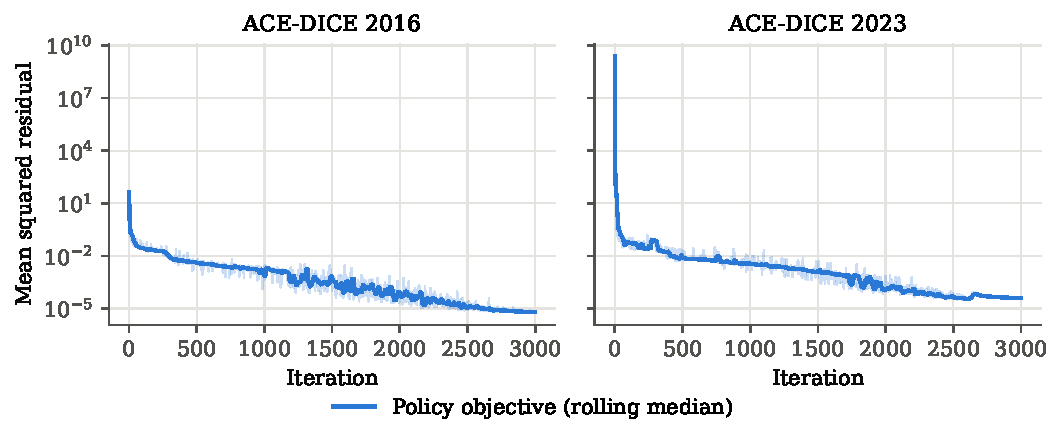
\includegraphics[width=1.0\textwidth]{images/ch6/revised/training_loss.pdf}
  \caption{Policy objective over training iterations (light line: per iteration; dark line: rolling median over 25 iterations)}
  \label{fig:training_loss}
\end{figure}

\subsubsection{Errors in Equilibrium Conditions}

The errors in the individual components that make up the total objective function, as given in equation (\ref{eq:total_objective_function}), are presented in Tables (\ref{table:errors2016}) and (\ref{table:errors-2023}), and summarized in Figure (\ref{fig:residuals}). The statistics in each column are the absolute errors \(|\ell_m|\) of the respective condition over an episode of 128 periods simulated with the best-performing network. The residuals are measured in the scaled units of section (\ref{subsubsec:objective_scaling}), so a residual of \(10^{-3}\) in \(\ell_1\) corresponds to an error of about \(10^{-3} \cdot c_M = 10^{-7}\) in the carbon costates, or about 0.1\% of their value.

\begin{table}[ht]
\centering
\begin{adjustbox}{width=\textwidth,center}
\begin{tabular}{lrrrrrrrrrrr}
\toprule
Statistic & $\ell_0$ & $\ell_{1,M_1}$ & $\ell_{1,M_2}$ & $\ell_{1,M_3}$ & $\ell_{2,\tau_1}$ & $\ell_{2,\tau_2}$ & $\ell_3$ & $\ell_4$ & $\ell_{5,A}$ & $\ell_{5,B}$ & $\ell_6$ \\
\midrule
mean & 2.4e-04 & 3.2e-04 & 1.4e-04 & 1.9e-05 & 2.3e-04 & 4.6e-05 & 2.4e-04 & 7.9e-04 & 4.4e-04 & 1.9e-04 & 7.9e-04 \\
std & 2.1e-04 & 2.6e-04 & 9.1e-05 & 1.3e-05 & 2.0e-04 & 4.4e-05 & 2.0e-04 & 7.8e-04 & 1.6e-03 & 1.7e-04 & 8.0e-04 \\
min & 9.8e-07 & 1.5e-06 & 2.0e-07 & 6.5e-07 & 4.5e-07 & 3.7e-08 & 2.5e-06 & 4.1e-06 & 9.5e-07 & 1.2e-06 & 7.6e-06 \\
25\% & 8.8e-05 & 1.3e-04 & 6.9e-05 & 9.2e-06 & 9.4e-05 & 1.7e-05 & 1.0e-04 & 2.8e-04 & 9.5e-07 & 5.9e-05 & 2.3e-04 \\
50\% & 1.9e-04 & 2.8e-04 & 1.4e-04 & 1.7e-05 & 1.8e-04 & 3.8e-05 & 2.1e-04 & 5.8e-04 & 1.1e-06 & 1.2e-04 & 5.6e-04 \\
75\% & 3.4e-04 & 4.1e-04 & 2.0e-04 & 2.8e-05 & 2.9e-04 & 5.5e-05 & 2.9e-04 & 1.0e-03 & 1.6e-04 & 2.9e-04 & 1.1e-03 \\
99.9\% & 1.2e-03 & 1.3e-03 & 5.1e-04 & 7.2e-05 & 1.1e-03 & 2.8e-04 & 9.2e-04 & 4.1e-03 & 1.4e-02 & 8.3e-04 & 4.0e-03 \\
max & 1.2e-03 & 1.3e-03 & 5.1e-04 & 7.5e-05 & 1.1e-03 & 2.8e-04 & 9.2e-04 & 4.1e-03 & 1.4e-02 & 8.3e-04 & 4.0e-03 \\
\bottomrule
\end{tabular}

\end{adjustbox}
\caption{Error Statistics ACE-DICE (2016 DICE), absolute errors \(|\ell_m|\)}
\label{table:errors2016}
\end{table}

\begin{table}[ht]
\centering
\begin{adjustbox}{width=\textwidth,center}
\begin{tabular}{lrrrrrrrrrrr}
\toprule
Statistic & $\ell_0$ & $\ell_{1,M_1}$ & $\ell_{1,M_2}$ & $\ell_{1,M_3}$ & $\ell_{2,\tau_1}$ & $\ell_{2,\tau_2}$ & $\ell_3$ & $\ell_4$ & $\ell_{5,A}$ & $\ell_{5,B}$ & $\ell_6$ \\
\midrule
mean & 1.7e-03 & 1.3e-03 & 4.4e-04 & 1.5e-05 & 8.1e-04 & 1.4e-04 & 1.4e-03 & 1.2e-03 & 8.6e-04 & 4.9e-04 & 2.3e-03 \\
std & 1.4e-03 & 8.9e-04 & 3.5e-04 & 1.3e-05 & 6.6e-04 & 1.3e-04 & 1.1e-03 & 1.4e-03 & 2.8e-03 & 3.8e-04 & 1.9e-03 \\
min & 6.9e-06 & 3.9e-05 & 3.5e-06 & 4.0e-08 & 3.4e-06 & 1.5e-06 & 1.9e-05 & 1.3e-05 & 9.5e-07 & 1.6e-06 & 7.6e-06 \\
25\% & 6.0e-04 & 6.3e-04 & 2.0e-04 & 5.9e-06 & 1.9e-04 & 5.2e-05 & 6.0e-04 & 3.7e-04 & 9.5e-07 & 1.7e-04 & 8.8e-04 \\
50\% & 1.3e-03 & 1.1e-03 & 3.1e-04 & 1.2e-05 & 6.7e-04 & 9.4e-05 & 1.1e-03 & 7.0e-04 & 1.1e-06 & 3.9e-04 & 1.6e-03 \\
75\% & 2.6e-03 & 1.8e-03 & 6.2e-04 & 2.2e-05 & 1.3e-03 & 1.6e-04 & 2.0e-03 & 1.7e-03 & 3.5e-04 & 8.1e-04 & 3.3e-03 \\
99.9\% & 5.8e-03 & 4.1e-03 & 1.7e-03 & 7.0e-05 & 2.8e-03 & 5.1e-04 & 5.2e-03 & 9.0e-03 & 2.3e-02 & 1.6e-03 & 8.2e-03 \\
max & 5.8e-03 & 4.1e-03 & 1.7e-03 & 7.1e-05 & 2.8e-03 & 5.1e-04 & 5.3e-03 & 9.3e-03 & 2.4e-02 & 1.7e-03 & 8.2e-03 \\
\bottomrule
\end{tabular}

\end{adjustbox}
\caption{Error Statistics ACE-DICE (2023 DICE), absolute errors \(|\ell_m|\)}
\label{table:errors-2023}
\end{table}

For the 2016 version, the mean absolute errors of all conditions lie between \(2 \cdot 10^{-5}\) and \(8 \cdot 10^{-4}\), and the maximum error over the episode is below \(5 \cdot 10^{-3}\) for every condition except the Fischer-Burmeister function \(\ell_{5,A}\). The largest errors are in the emissions condition \(\ell_4\) and the Bellman equation \(\ell_6\). The errors for the 2023 version are mostly larger, by up to a factor of seven, but the maximum error remains below \(10^{-2}\) for every condition except \(\ell_{5,A}\). For the consumption condition \(\ell_3\) and the Bellman equation \(\ell_6\), which are measured in the same units as in the original implementation, the mean errors are about two orders of magnitude smaller than before. The comparison is only indicative, as the original errors measured residuals of different, partly incorrect, conditions.

The largest errors of \(\ell_{5,A}\) occur at the few periods in which the analytical abatement rate reaches one and the constraint \(E_t \geq 0\) starts to bind, around 2175 for the 2016 version and 2190 for the 2023 version. There, the complementarity condition switches between its two branches, which the smooth policy network can only approximate, and the median error of \(\ell_{5,A}\) is about \(10^{-6}\) in both versions.

\begin{figure}[ht]
  \centering
  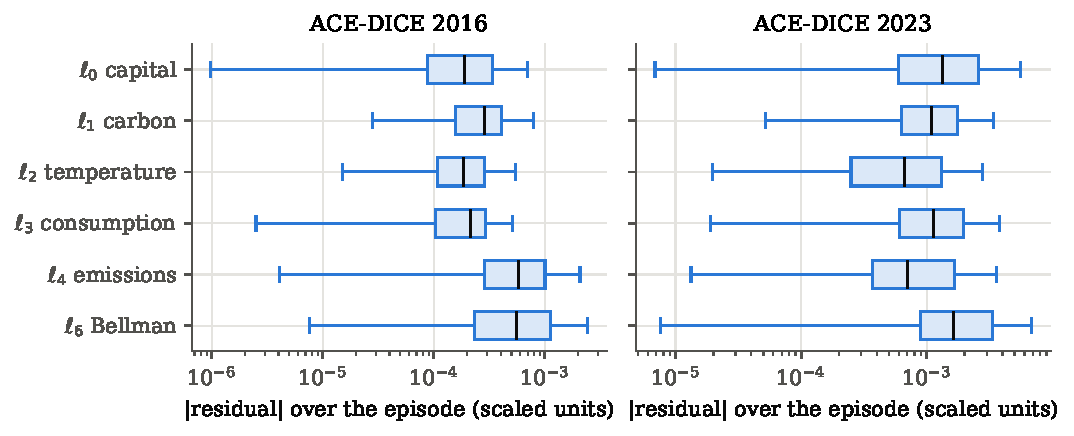
\includegraphics[width=1.0\textwidth]{images/ch6/revised/residuals.pdf}
  \caption{Distribution of the absolute errors over the simulated episode. For conditions with several components, the largest component in each period is shown. Boxes show the interquartile range, whiskers the full range.}
  \label{fig:residuals}
\end{figure}


\subsection{Analytical Comparisons}

This section compares the simulated results with the analytical solution of ACE. I begin with the consumption rate and the abatement rate, continue with the costate variables and the SCC they imply, and end with the simulated paths of the states. Throughout, the figures show the paths up to the year 2300, and the policy network is evaluated along its own simulated trajectory. Table (\ref{table:comparison}) summarizes the main comparisons.

\begin{table}[ht]
\centering
\begin{adjustbox}{width=\textwidth,center}
\begin{tabular}{lcccc}
\toprule
 & \multicolumn{2}{c}{ACE-DICE 2016} & \multicolumn{2}{c}{ACE-DICE 2023} \\
\cmidrule(lr){2-3} \cmidrule(lr){4-5}
 & DEQN & Analytic & DEQN & Analytic \\
\midrule
Consumption rate $x$ (mean to 2300) & 0.7394 & 0.7395 & 0.7396 & 0.7395 \\
Costate $\lambda_k$ & 0.3524 & 0.3524 & 0.3520 & 0.3524 \\
Costate $\lambda_{M_1}$ ($\times 10^{-4}$) & -1.046 & -1.046 & -1.044 & -1.046 \\
Costate $\lambda_{\tau_1}$ & -0.0559 & -0.0559 & -0.0559 & -0.0559 \\
SCC in 2050 (USD/tCO$_2$) & 36.9 & 37.0 & 37.3 & 37.4 \\
Temperature in 2100 (°C) & 2.96 & 2.96 & 3.47 & 3.47 \\
Peak temperature (°C) & 3.33 & 3.33 & 4.71 & 4.72 \\
\midrule
Abatement rate, mean $|\mu - \mu^*|$ & \multicolumn{2}{c}{0.0009} & \multicolumn{2}{c}{0.0020} \\
Abatement rate, max $|\mu - \mu^*|$ & \multicolumn{2}{c}{0.0166} & \multicolumn{2}{c}{0.0227} \\
\bottomrule
\end{tabular}

\end{adjustbox}
\caption{Policy network (DEQN) against the analytical solution. Costates are averaged over the periods up to 2300; the abatement rate errors are taken over the same periods.}
\label{table:comparison}
\end{table}

\subsubsection{The Consumption Rate}

As shown in equation (\ref{eq:analytical_x_t}), the optimal consumption rate is constant over time and independent of the states visited, \(x^* = 1 - \beta\kappa \approx 0.7395\). The upper panels of Figure (\ref{fig:controls}) show the consumption rates estimated by the policy network, together with the analytical rate and the consumption rates estimated with the original implementation.

\begin{figure}[ht]
  \centering
  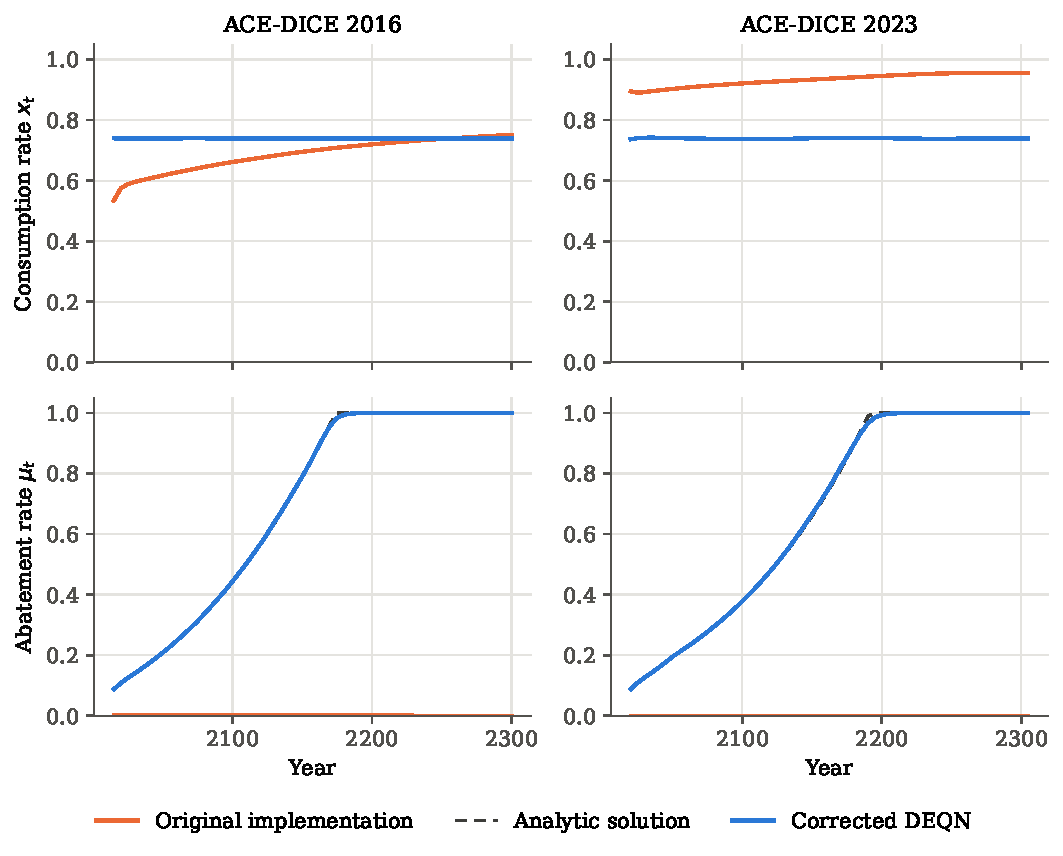
\includegraphics[width=1.0\textwidth]{images/ch6/revised/controls.pdf}
  \caption{Consumption rate (top) and abatement rate (bottom): corrected DEQN, analytical solution and original implementation}
  \label{fig:controls}
\end{figure}

The estimated consumption rates match the analytical solution closely. Over the periods up to 2300, the largest deviation from \(x^*\) is \(6 \cdot 10^{-4}\) for the 2016 version and \(2.8 \cdot 10^{-3}\) for the 2023 version, and the policy network has learned that the consumption rate does not depend on the state. In contrast, the original implementation estimated a consumption rate that rises from about 0.53 to 0.75 for the 2016 version and lies above 0.89 for the 2023 version. These deviations were not caused by the normalization of inputs, as suggested in the submitted version of this thesis, but by the errors in the capital condition \(\ell_0\) and the consumption condition \(\ell_3\): at the analytical solution, the original conditions are not zero, so the network was trained towards a different fixed point.

\subsubsection{The Abatement Rate}

Given the carbon price implied by the costate variables, the optimal abatement rate solves the first-order condition on emissions (eq. \ref{eq:general_objective_4}), which is equivalent to equation (\ref{eq:analytical_abatement_rate}) with \(\Gamma_t = SCC_t\). Where the solution exceeds one, the constraint \(E_t \geq 0\) binds and the abatement rate is one.

The lower panels of Figure (\ref{fig:controls}) show that the estimated abatement rates follow the analytical rates closely, from about 9\% in the first period to full abatement in 2175 for the 2016 version and in 2195 for the 2023 version. The mean absolute deviation over the periods up to 2300 is 0.0009 for the 2016 version and 0.0020 for the 2023 version. The largest deviations, of about 0.02, occur in the few periods around the kink where the abatement rate reaches one, which the smooth policy network rounds off. The original implementation estimated abatement rates close to zero in both versions.

\subsubsection{Costate Variables and the Social Cost of Carbon}

The costate variables of ACE are constant along the optimal path (Appendix \ref{appendix:supplementary_figures}). The policy network recovers them with a largest relative deviation over the periods up to 2300 of 0.3\% for \(\lambda_k\), 0.5\% for \(\lambda_{M_1}\) and 0.4\% for \(\lambda_{\tau_1}\) in the 2016 version, and of 1.4\%, 1.4\% and 0.5\% in the 2023 version. This is notable for the carbon costate \(\lambda_{M_1} \approx -1.05 \cdot 10^{-4}\), which is four orders of magnitude smaller than \(\lambda_k\) and is only identified through the conditions on the carbon cycle and on emissions. Without the scaling of section (\ref{subsubsec:objective_scaling}), these conditions carry almost no weight in the policy objective.

\begin{figure}[ht]
  \centering
  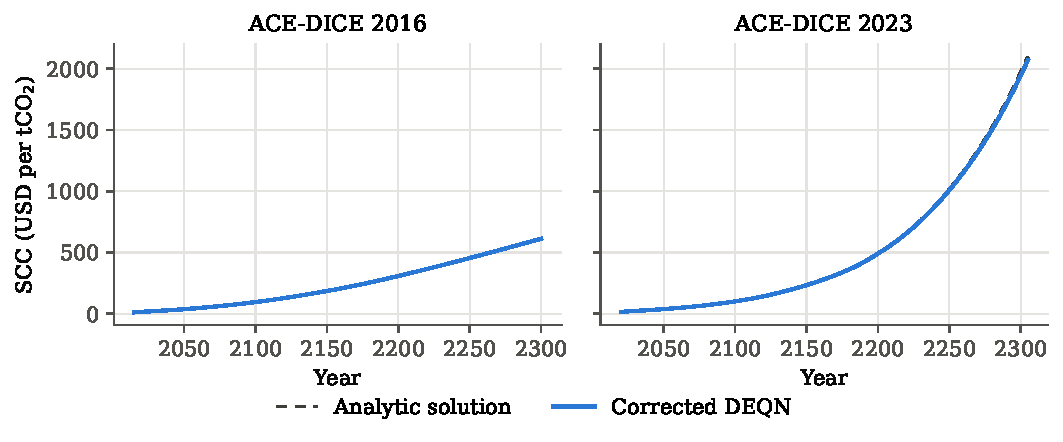
\includegraphics[width=1.0\textwidth]{images/ch6/revised/scc.pdf}
  \caption{SCC in USD/tCO$_2$ implied by the policy network and the analytical solution}
  \label{fig:social_cost_of_carbon_plot}
\end{figure}

Figure (\ref{fig:social_cost_of_carbon_plot}) shows the SCC implied by the costates of the policy network, as given below equation (\ref{eq:analytical_scc}), together with the analytical SCC (eq. \ref{eq:analytical_scc}) evaluated at the same states. The two are almost indistinguishable. For the 2016 version, the SCC rises from 11.1 USD/tCO\(_2\) in 2015 (analytical: 11.0) to 95.1 USD/tCO\(_2\) in 2100 (95.1). For the 2023 version, it rises from 14.1 USD/tCO\(_2\) in 2020 (14.2) to 100.5 USD/tCO\(_2\) in 2100 (100.9). The SCC is proportional to net output, so it grows faster in the 2023 version, where total factor productivity grows faster.

\subsubsection{Simulated Paths}

Figure (\ref{fig:states}) compares the states along the trajectory simulated with the policy network to the optimal path obtained by simulating the analytical controls from the same initial state. Since the estimated controls are close to optimal, the two paths coincide. In the 2016 version, atmospheric temperature peaks at 3.33°C around 2150 and atmospheric carbon at about 1590 GtC. In the 2023 version, where emissions are higher because of faster output growth, temperature peaks at 4.71°C around 2185 (analytical: 4.72°C). The small differences after 2200 in the 2023 version reflect the deviations in the abatement rate around the kink.

\begin{figure}[ht]
  \centering
  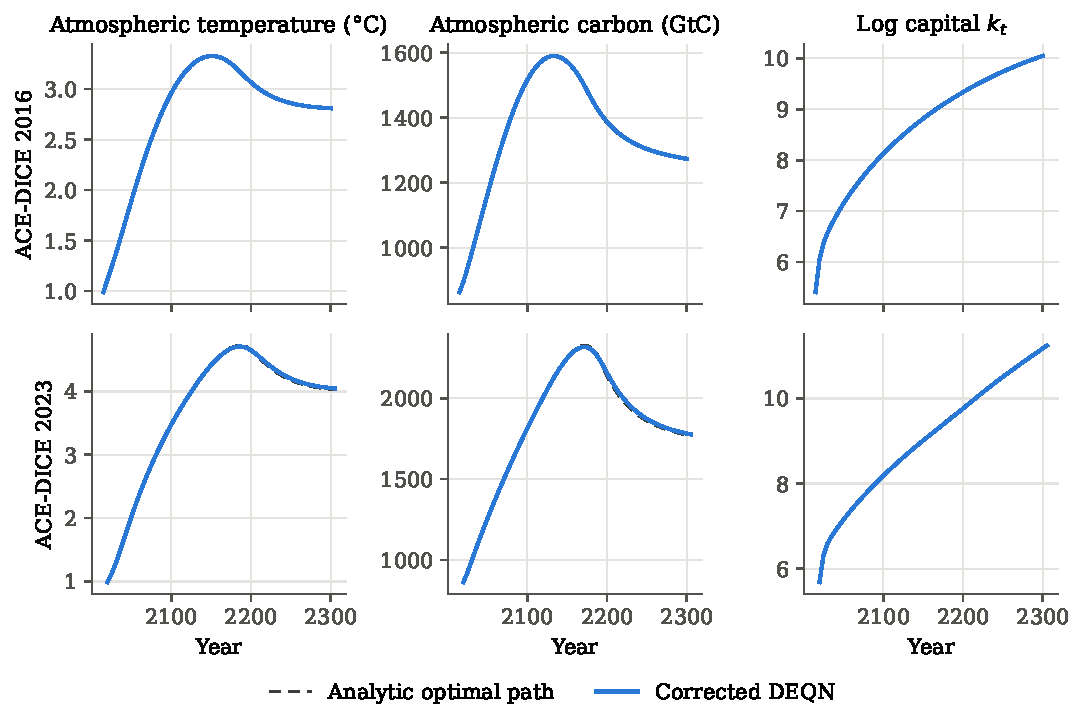
\includegraphics[width=1.0\textwidth]{images/ch6/revised/states.pdf}
  \caption{Atmospheric temperature, atmospheric carbon and log capital along the trajectory simulated with the policy network and along the analytical optimal path}
  \label{fig:states}
\end{figure}
